% File : rev_literatura.tex


\chapter{Comparações}

blablalbalbalbalbalbalblablalbbbbbblbalbalbalblalbalbalblalbalblaba
blablalbalbalbalbalbalblablalbbbbbblbalbalbalblalbalbalblalbalblaba
blablalbalbalbalbalbalblablalbbbbbblbalbalbalblalbalbalblalbalblabal
albalblablablalbla

%%%%%%%%%%%%%%%%%%%%%%%%%%%%%%%%%%%%%%%%%%%%%%%%%%%%%%%%%%%%%%%%%%%%%%%%%%%%%%%%%%%%%%%%%%%%%%%%%%%%%%%%%%%
%%%%%%%%%%%%%%%%%%%%%%%%%%%%%%%%%%%% AFAZERES_DOM %%%%%%%%%%%%%%%%%%%%%%%%%%%%%%%%%%%%%%%%%%%%%%%%%%%%%%%%%
%%%%%%%%%%%%%%%%%%%%%%%%%%%%%%%%%%%%%%%%%%%%%%%%%%%%%%%%%%%%%%%%%%%%%%%%%%%%%%%%%%%%%%%%%%%%%%%%%%%%%%%%%%%
\section{Tempo de afazeres domésticos}

blablalbalbalbalbalbalblablalbbbbbblbalbalbalblalbalbalblalbalblaba
blablalbalbalbalbalbalblablalbbbbbblbalbalbalblalbalbalblalbalblaba
blablalbalbalbalbalbalblablalbbbbbblbalbalbalblalbalbalblalbalblabal
albalblablablalbla


%%%%%%%%%%%%%%%%%%%%%%% Graficos %%%%%%%%%%%%%%%%%%%%%%%%%%%%%%%%%%%%%%%%%%%%%%%%%%%%%%%%%%%%%%%%%
\newpage
%%%%% Gráfico de Sexo por afazeres_domesticos
\begin{figure}[h]
    \caption{Proporção por sexo de tempos de afazeres domésticos por parte
    dos alunos.}
    \begin{center}
        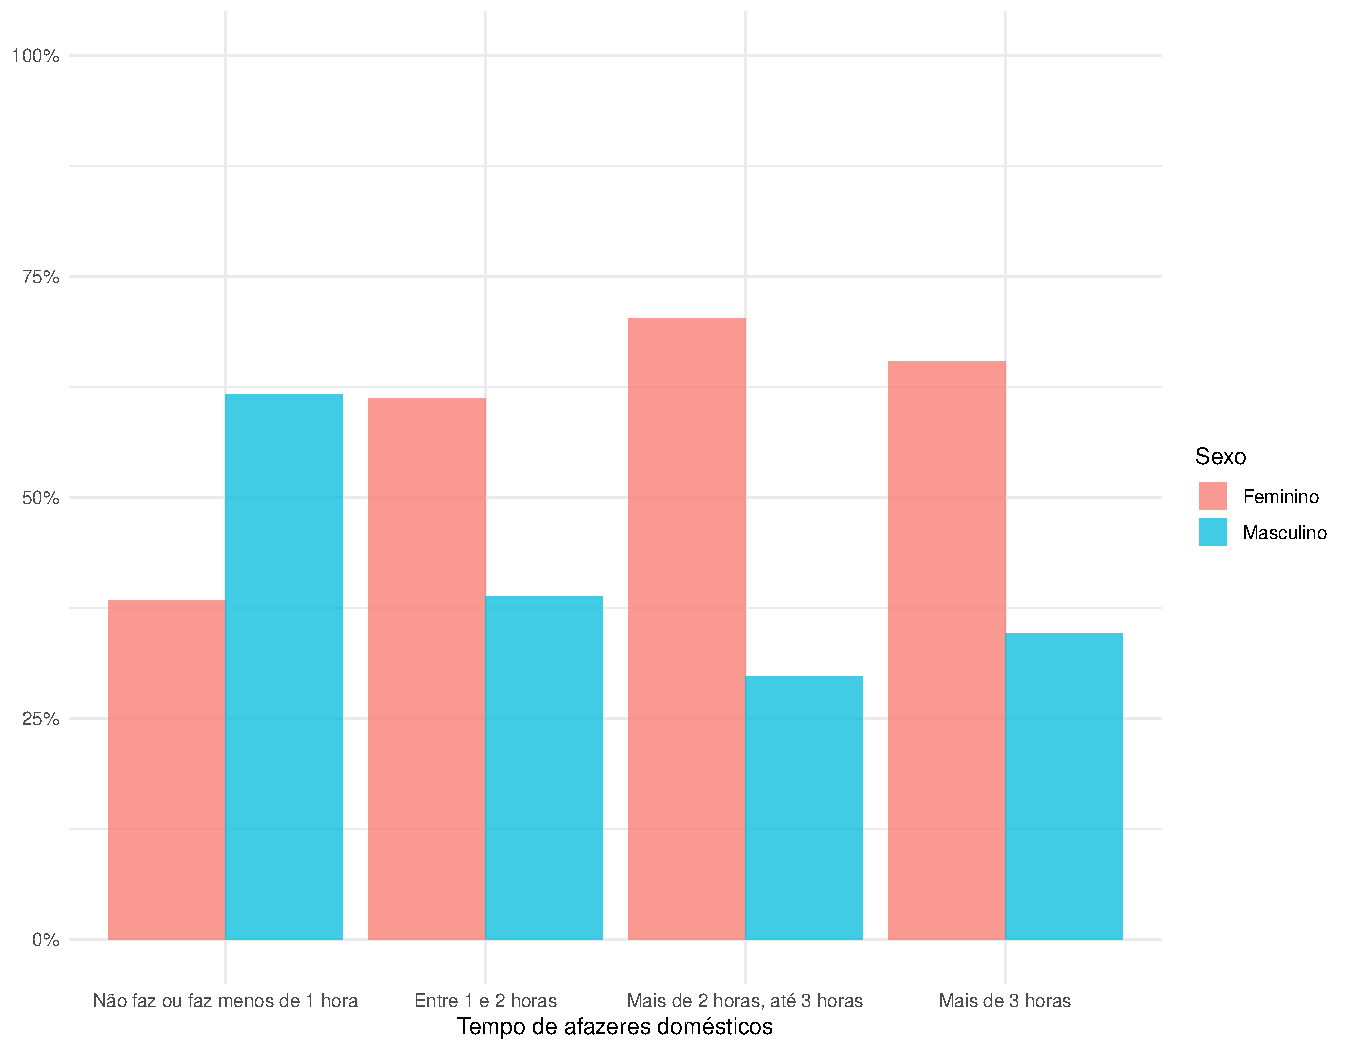
\includegraphics[width=16cm]{img/sexo_afazeres.pdf}
    \end{center}
    \fonte{Amostra de 5271 alunos do 9º ano do SAEB 2017.}
    \nota{Amostra retirada de uma amostragem aleatórias simples.}
\end{figure}

%%%%% Gráfico de Escolaridade da mãe por afazeres_domesticos
%\begin{figure}[h]
%    \caption{Proporção por sexo de tempos de afazeres domésticos por parte
%    dos alunos.}
%    \begin{center}
%        \includegraphics[width=16cm]{img/}
%    \end{center}
%    \fonte{Amostra de 5271 alunos do 9º ano do SAEB 2017.}
%    \nota{Amostra retirada de uma amostragem aleatórias simples.}
%\end{figure}


%%%%%%%%%%%%%%%%%%%%%%% Tabelas %%%%%%%%%%%%%%%%%%%%%%%%%%%%%%%%%%%%%%%%%%%%%%%%%%%%%%%%%%%%%%%%%

\newpage
%%%%% Tabela dos testes paras relações com afazeres domesticos
\begin{table}[htb]
    \caption{Testes de igualdade na variabilidade sobre as relações 
            com o tempo de afazeres domésticos por parte dos alunos.}
        \centering
        \begin{tabular}{cccc}
        \toprule
        Teste & $H_0$& P-valor & Decisão de $H_0$ (95\%)\\
        \midrule \midrule
        K & $\mu_{Raça/Cor}$ iguais & 0.369 & Aceita\\
        K & $\mu_{Esc(mãe)}$ iguais & Aprox. 0 & Rejeita\\
        K & $\mu_M = \mu_F$ iguais & Aprox. 0 & Rejeita\\
        \bottomrule
        \end{tabular}
        \fonte{Amostra de 5271 alunos do 9º ano do SAEB 2017.}
        \nota{Amostra retiradas de uma amostragem aleatórias simples.}
        \nota[Anotações]{Os subíndices M e F refere-se aos sexos Masculino e Feminino
        dos alunos respectivamente. O Aprox. 0 refere-se à algum número muito pequeno considerado
         por este estudo aproximadamente zero.}
\end{table}


\newpage
%%%%% Tabela de comparação da escolaridade da mãe com afazeres domesticos
\begin{table}[htb]
    \centering
\caption{Comparações dois a dois entre as ordens das posições sobre os tempos de afazeres domésticos
com base na escolaridade das mães dos alunos.}
    \begin{tabular}{lcc}
    \toprule
    Comparações & P-valor & Evidência (RA 95\%)\\
    \midrule \midrule
    Não sabe = Nunca estudou & Aprox. 0 & Desiguais\\
    Não sabe = Incompleto 5.º ano do EF  & 1.0000 & Iguais\\
    Não sabe = Completou 5.º ano do EF  & 0.0084 & Desiguais\\
    Não sabe = Completou 9.º ano do EF  & 0.1927 & Iguais\\
    Não sabe = Completou EM & Aprox. 0 & Desiguais\\
    Não sabe = Completou Faculdade & Aprox. 0 & Desiguais\\
    Nunca estudou = Incompleto 5.º ano do EF  & 0.0038 & Desiguais\\
    Nunca estudou = Completou 5.º ano do EF  & Aprox. 0 & Desiguais\\
    Nunca estudou = Completou 9.º ano do EF  & Aprox. 0 & Desiguais\\
    Nunca estudou = Completou EM & Aprox. 0 & Desiguais\\
    Nunca estudou = Completou Faculdade & Aprox. 0 & Desiguais\\
    Incompleto 5.º ano do EF = Completou 5.º ano do EF  & 0.0002 & Desiguais\\
    Incompleto 5.º ano do EF = Completou 9.º ano do EF  & 0.0048 & Desiguais\\
    Incompleto 5.º ano do EF = Completou EM & Aprox. 0 & Desiguais\\
    Incompleto 5.º ano do EF = Completou Faculdade & Aprox. 0 & Desiguais\\
    Completo 5.º ano do EF = Completou 9.º ano do EF  & 1 & Iguais\\
    Completo 5.º ano do EF = Completou EM & Aprox. 0 & Desiguais\\
    Completo 5.º ano do EF = Completou Faculdade & Aprox. 0 & Desiguais\\
    Completo 9.º ano do EF = Completou EM & Aprox. 0 & Desiguais\\
    Completo 9.º ano do EF = Completou Faculdade & Aprox. 0 & Desiguais\\
    Completou EM = Completou Faculdade & 1.0000 & Iguais\\
    \bottomrule
    \end{tabular}
    \centering
    \fonte{Amostra de 5271 alunos do 9º ano do SAEB 2017.}
    \nota{Amostra retiradas de uma amostragem aleatórias simples.}
    \nota[Anotações]{Aprox. 0 refere-se à algum número muito pequeno considerando aproximadamente zero.}
    
\end{table}




\newpage
%%%%%%%%%%%%%%%%%%%%%%%%%%%%%%%%%%%%%%%%%%%%%%%%%%%%%%%%%%%%%%%%%%%%%%%%%%%%%%%%%%%%%%%%%%%%%%%%%%%%%%%%%%%
%%%%%%%%%%%%%%%%%%%%%%%%%%%%%%%%% NOTAS %%%%%%%%%%%%%%%%%%%%%%%%%%%%%%%%%%%%%%%%%%%%%%%%%%%%%%%%%%%%%%%%%%%%%%%%%
%%%%%%%%%%%%%%%%%%%%%%%%%%%%%%%%%%%%%%%%%%%%%%%%%%%%%%%%%%%%%%%%%%%%%%%%%%%%%%%%%%%%%%%%%%%%%%%%%%%%%%%%%%%
\section{Notas}

blablalbalbalbalbalbalblablalbbbbbblbalbalbalblalbalbalblalbalblaba
blablalbalbalbalbalbalblablalbbbbbblbalbalbalblalbalbalblalbalblaba
blablalbalbalbalbalbalblablalbbbbbblbalbalbalblalbalbalblalbalblabal
albalblablablalbla

%%%%%%%%%%%%%%%%%%%%%%% Graficos %%%%%%%%%%%%%%%%%%%%%%%%%%%%%%%%%%%%%%%%%%%%%%%%%%%%%%%%%%%%%%%%%
\newpage
%%%%% Grafico com raca cor e notas
\begin{figure}[h]
    \caption{Distribuições das somas das notas com base na raça/cor dos alunos.}
    \begin{center}
        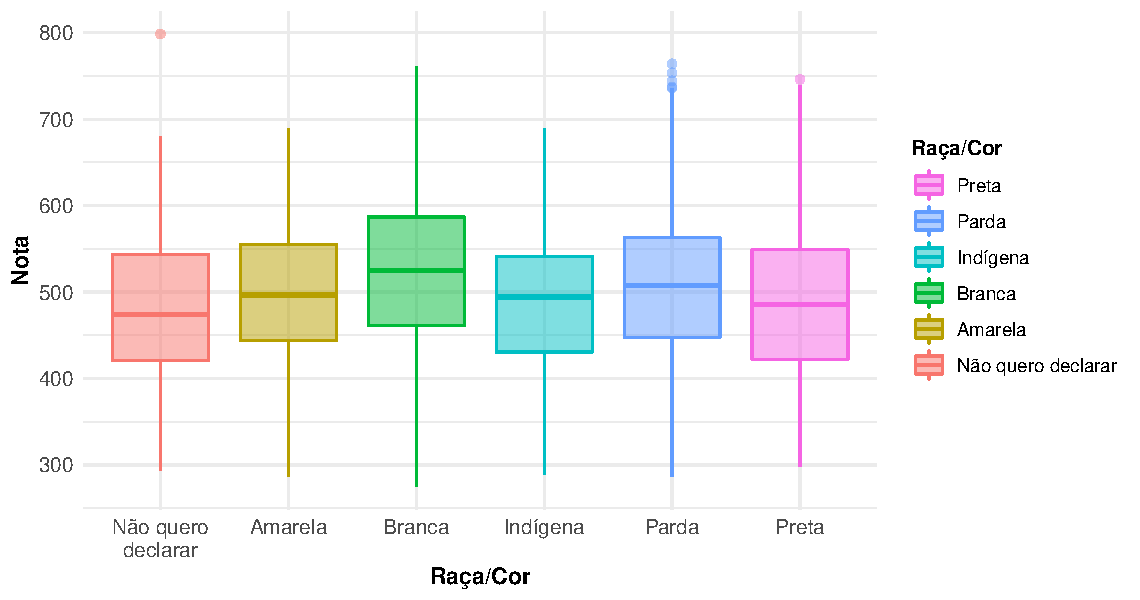
\includegraphics[width=16cm]{img/raca_cor_notas.pdf}
    \end{center}
    \fonte{Amostra de 5271 alunos do 9º ano do SAEB 2017.}
    \nota{Amostra retirada de uma amostragem aleatórias simples.}
\end{figure}


\newpage
%%%% Grafico localizacao com notas
\begin{figure}[htb]
    \caption{Distribuições empíricas das somas das notas com base nas localizações das
    das escolas dos alunos.}
    \begin{center}
        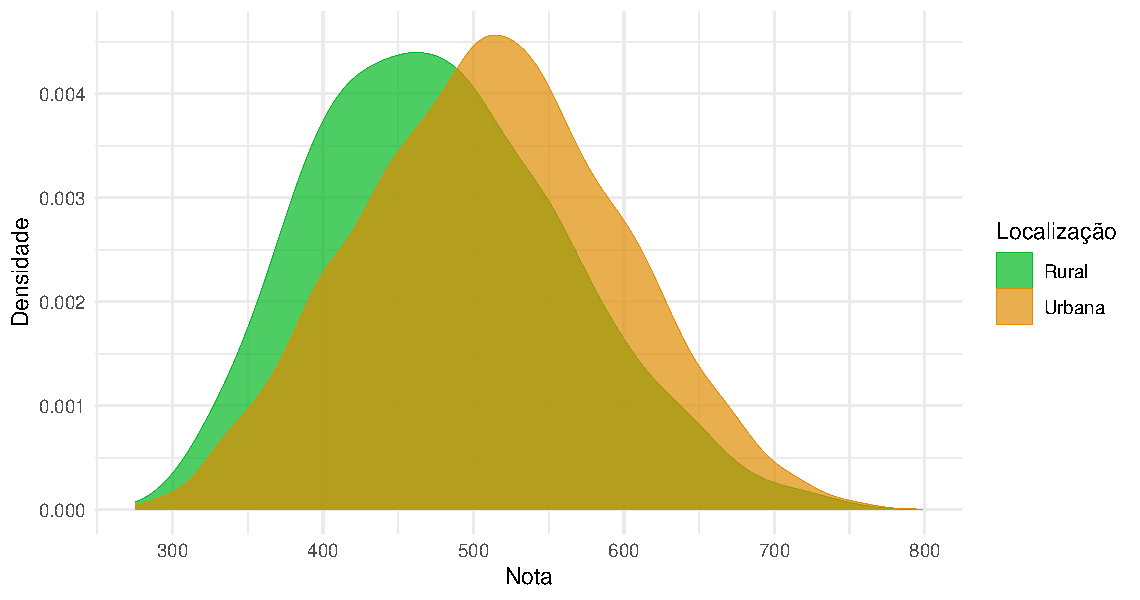
\includegraphics[width=16cm]{img/loc_notas.pdf}
    \end{center}
    \fonte{Amostra de 5271 alunos do 9º ano do SAEB 2017.}
    \nota{Amostra retirada de uma amostragem aleatórias simples.}
\end{figure}


\newpage
%%%%% Grafico da escolaridade da mae com notas
\begin{figure}[h]
    \caption{Distribuições das somas das notas com base nas escolaridades 
    das mães dos alunos.}
    \begin{center}
        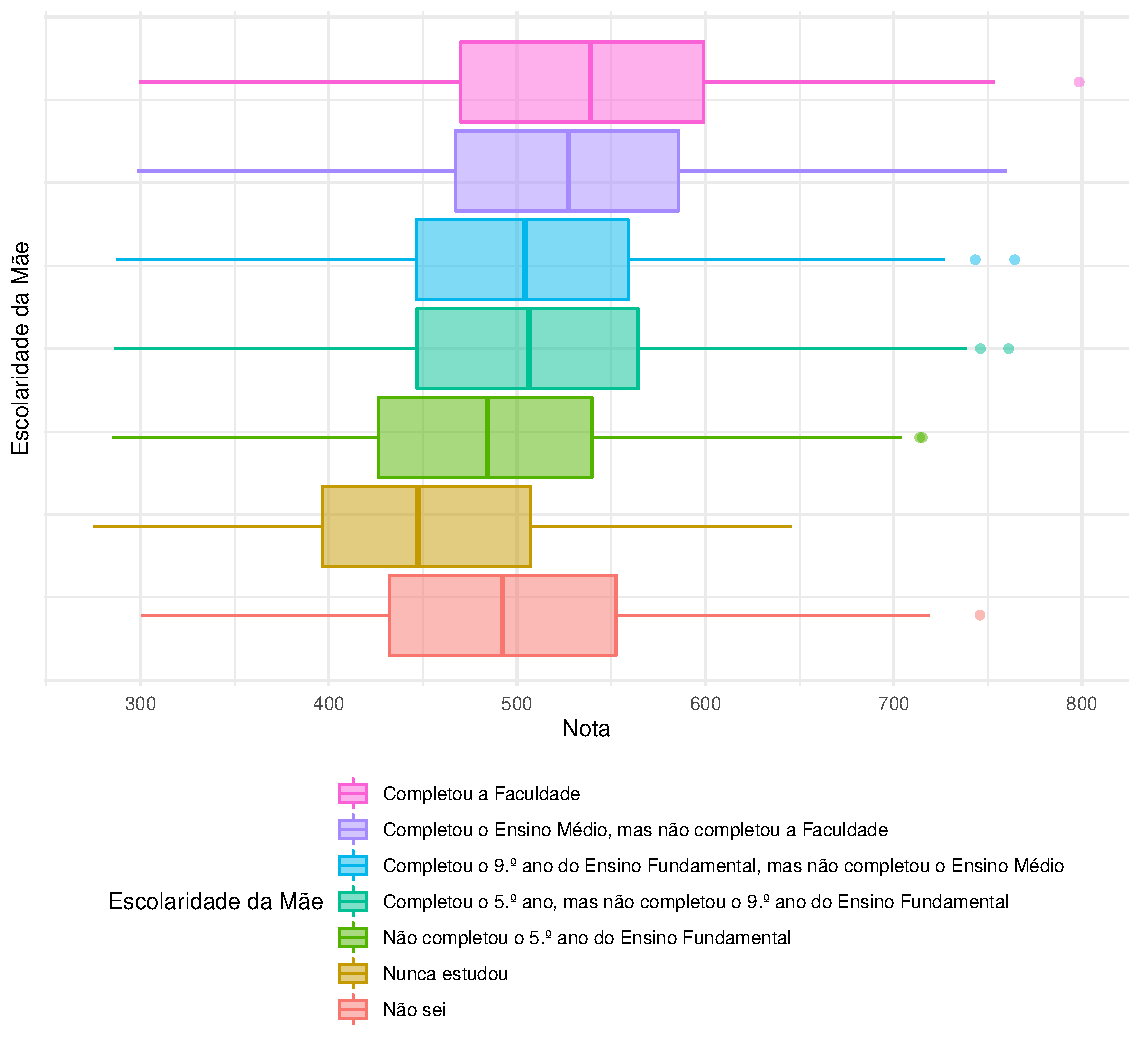
\includegraphics[width=16cm]{img/esc_mae_notas.pdf}
    \end{center}
    \fonte{Amostra de 5271 alunos do 9º ano do SAEB 2017.}
    \nota{Amostra retirada de uma amostragem aleatórias simples.}
\end{figure}




%%%%%%%%%%%%%%%%%%%%%%% Tabelas %%%%%%%%%%%%%%%%%%%%%%%%%%%%%%%%%%%%%%%%%%%%%%%%%%%%%%%%%%%%%%%%%
\newpage
%%%%%% Tabela com testes para as relacoes das notas
\begin{table}[htb]
\caption{Testes para as relações com soma
 das notas dos alunos.}
    \centering
    \begin{tabular}{cccc}
    \toprule
    Teste & $H_0$& P-valor & Decisão de $H_0$ (95\%)\\
    \midrule \midrule
    B & $\sigma_R^2 = \sigma_U^2$ & 0.503 & Aceita\\
    B & $\sigma_{Raça/Cor}^2$ iguais & 0.265 & Aceita\\
    B & $\sigma_{Esc(mãe)}^2$ iguais & 0.132 & Aceita\\
    ANOVA & $\mu_R^2 = \mu_U^2$ iguais & Aprox. 0 & Rejeita\\
    ANOVA & $\mu_{Raça/Cor}$ iguais & Aprox. 0 & Rejeita\\
    ANOVA & $\mu_{Esc(mãe)}$ iguais & Aprox. 0 & Rejeita\\
    \bottomrule
    \end{tabular}
    \fonte{Amostra de 5271 alunos do 9º ano do SAEB 2017.}
    \nota{Amostra retiradas de uma amostragem aleatórias simples.}
    \nota[Anotações]{Os subíndices $R$ e $U$ refere-se as localizações
                    das escolas rurais e urbanas respectivamente. O Aprox. 0 refere-se à algum número 
                    muito pequeno considerado por este estudo aproximadamente zero.}
\end{table}

\newpage
%%%%%% Tabela de comparacao entre raca/cor e notas
\begin{table}[htb]
    \centering
\caption{Comparações dois a dois entre as médias sobre a soma das notas
        com base na raça/cor dos alunos.}
    \begin{tabular}{lcc}
    \toprule
    Comparações & P-valor & Evidência (RA 95\%)\\
    \midrule \midrule
    Amarela = Não quero declarar & 0.4113 & Iguais\\
    Amarela = Branca & 0.0005 & Desiguais\\
    Amarela = Indígena & 1.0000 & Iguais\\
    Amarela = Parda & 1.0000 & Iguais\\
    Amarela = Preta & 1.0000 & Iguais\\
    Branca = Não quero declarar & Aprox. 0 & Desiguais\\
    Branca = Indígena & 0.0010 & Desiguais\\
    Branca = Parda & Aprox. 0 & Desiguais\\
    Branca = Preta & Aprox. 0 & Desiguais\\
    Indígena = Não quero declarar & 1.0000 & Iguais\\
    Indígena = Parda & 0.7758 & Iguais\\
    Indígena = Preta & 1.0000  & Iguais\\
    Parda = Não quero declarar & Aprox. 0 & Desiguais\\
    Parda = Preta & Aprox. 0 & Desiguais\\
    \bottomrule
    \end{tabular}
    \centering
    \fonte{Amostra de 5271 alunos do 9º ano do SAEB 2017.}
    \nota{Amostra retiradas de uma amostragem aleatórias simples.}
    \nota[Anotações]{Aprox. 0 refere-se à algum número muito pequeno considerando aproximadamente zero.}
    
\end{table}


\newpage
%%%%% Tabela de comparação da notas com Escolaridade da mae
\begin{table}[htb]
    \centering
\caption{\label{comp_MT}Comparações entre as médias de notas em Matemática e as regiões das escolas dos alunos com base na amostra de tamanho 500.}
    \begin{tabular}{lcc}
    \toprule
    Comparações & P-valor & Evidência (RA 95\%)\\
    \midrule \midrule
    Não sabe = Nunca estudou & 1.0000 & Iguais\\
    Não sabe = Incompleto 5.º ano do EF  & 0.0078 & Desiguais\\
    Não sabe = Completou 5.º ano do EF  & 0.0005 & Desiguais\\
    Não sabe = Completou 9.º ano do EF  & 0.0001 & Desiguais\\
    Não sabe = Completou EM & Aprox. 0 & Desiguais\\
    Não sabe = Completou Faculdade & 0.0011 & Desiguais\\
    Nunca estudou = Incompleto 5.º ano do EF  & 1.0000 & Iguais\\
    Nunca estudou = Completou 5.º ano do EF  & 0.5598 & Iguais\\
    Nunca estudou = Completou 9.º ano do EF  & 0.4165 & Iguais\\
    Nunca estudou = Completou EM & 0.1114 & Iguais\\
    Nunca estudou = Completou Faculdade & 0.4707 & Iguais\\
    Incompleto 5.º ano do EF = Completou 5.º ano do EF  & 1.0000 & Iguais\\
    Incompleto 5.º ano do EF = Completou 9.º ano do EF  & 1.0000 & Iguais\\
    Incompleto 5.º ano do EF = Completou EM & 1.0000 & Iguais\\
    Incompleto 5.º ano do EF = Completou Faculdade & 1.0000 & Iguais\\
    Completo 5.º ano do EF = Completou 9.º ano do EF  & 1.0000 & Iguais\\
    Completo 5.º ano do EF = Completou EM & 1.0000 & Iguais\\
    Completo 5.º ano do EF = Completou Faculdade & 1.0000 & Iguais\\
    Completo 9.º ano do EF = Completou EM & 1.0000 & Iguais\\
    Completo 9.º ano do EF = Completou Faculdade & 1.0000 & Iguais\\
    Completou EM = Completou Faculdade & 1.0000 & Iguais\\
    \bottomrule
    \end{tabular}
    \centering
    \fonte{Amostra de 5271 alunos do 9º ano do SAEB 2017.}
    \nota{Amostra retiradas de uma amostragem aleatórias simples.}
    \nota[Anotações]{Aprox. 0 refere-se à algum número muito pequeno considerando aproximadamente zero.}
    
\end{table}
